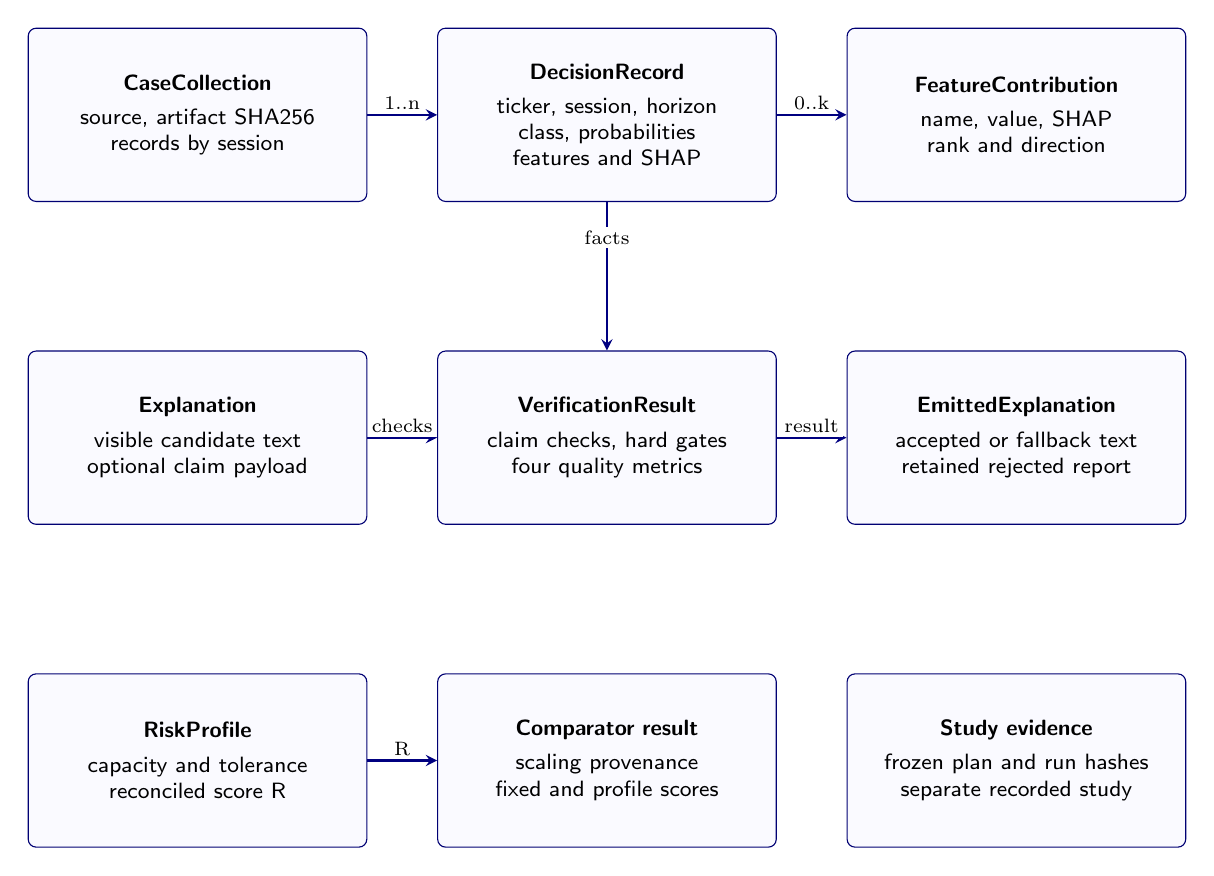
\begin{tikzpicture}[x=1mm,y=1mm,box/.style={draw=blue!45!black,fill=blue!2,rounded corners=1mm,align=center,text width=39mm,minimum height=22mm,inner sep=2mm,font=\sffamily\footnotesize},link/.style={->,>=stealth,draw=blue!50!black,thick}]
\node[box] (collection) at (23,100) {\textbf{CaseCollection}\\[1mm]source, artifact SHA256\\records by session};
\node[box] (record) at (75,100) {\textbf{DecisionRecord}\\[1mm]ticker, session, horizon\\class, probabilities\\features and SHAP};
\node[box] (contrib) at (127,100) {\textbf{FeatureContribution}\\[1mm]name, value, SHAP\\rank and direction};
\node[box] (explanation) at (23,59) {\textbf{Explanation}\\[1mm]visible candidate text\\optional claim payload};
\node[box] (verification) at (75,59) {\textbf{VerificationResult}\\[1mm]claim checks, hard gates\\four quality metrics};
\node[box] (emission) at (127,59) {\textbf{EmittedExplanation}\\[1mm]accepted or fallback text\\retained rejected report};
\node[box] (profile) at (23,18) {\textbf{RiskProfile}\\[1mm]capacity and tolerance\\reconciled score R};
\node[box] (comparison) at (75,18) {\textbf{Comparator result}\\[1mm]scaling provenance\\fixed and profile scores};
\node[box] (study) at (127,18) {\textbf{Study evidence}\\[1mm]frozen plan and run hashes\\separate recorded study};
\draw[link] (collection.east) -- (record.west) node[pos=.5,above,fill=white,inner sep=.5mm,font=\scriptsize]{1..n};
\draw[link] (record.east) -- (contrib.west) node[pos=.5,above,fill=white,inner sep=.5mm,font=\scriptsize]{0..k};
\draw[link] (record.south) -- ++(0,-6) -| (verification.north) node[pos=.5,above,fill=white,inner sep=.5mm,font=\scriptsize]{facts};
\draw[link] (explanation.east) -- (verification.west) node[pos=.5,above,fill=white,inner sep=.5mm,font=\scriptsize]{checks};
\draw[link] (verification.east) -- (emission.west) node[pos=.5,above,fill=white,inner sep=.5mm,font=\scriptsize]{result};
\draw[link] (profile.east) -- (comparison.west) node[pos=.5,above,fill=white,inner sep=.5mm,font=\scriptsize]{R};
\end{tikzpicture}
